\section{Deep Convolutional Neural Networks}
\label{sec:networks}

This section briefly presents the deep \ac{cnn} architectures used in this work. Furthermore, the image preprocessing and training details are described.



% The method presented in this paper does not utilize document features that require a high resolution, such as optical character recognition. Instead, it solely relies on the structure and layout of the input documents to classify them. Therefore, in a preprocessing step, the high-resolution images are downscaled to a lower resolution of $227\times227$ which is the input size of the CNN.

% The common approach to successfully train CNNs for object recognition is to augment the training data by resizing the images to a larger size and to then randomly crop areas from these images (\cf \cite{cnn_alexnet_nips2014}). This data augmentation technique has proven to be effective for networks trained on the ImageNet data set where the most discriminating elements of the images are typically located close to the center of the image and therefore contained in all crops. However, by this technique the network is effectively presented with less than 80\% of the original image. We intentionally do not augment our training data in this way, because unlike in object recognition, the most discriminating parts of document images often reside in the outer regions of the document, \eg the head of a letter.

% As a second preprocessing step, we subtract the mean values of the training images from both the training and the validation images.

% Lastly, we convert the grayscale document images to RGB images, \ie we copy the values of the single-channel images to generate three-channel images. 

% ToDo, Discuss: Why is this important?

% The original weights which are used to initialize the proposed network were trained using all three channels RGB and therefore extracts different types of features. We introduce the same information in all the channels in order to enrich the features for better classification.


% \subsection{Network Architectures}
% \begin{figure*}
%     \begin{subfigure}{0.23\linewidth}
%         \centering
%         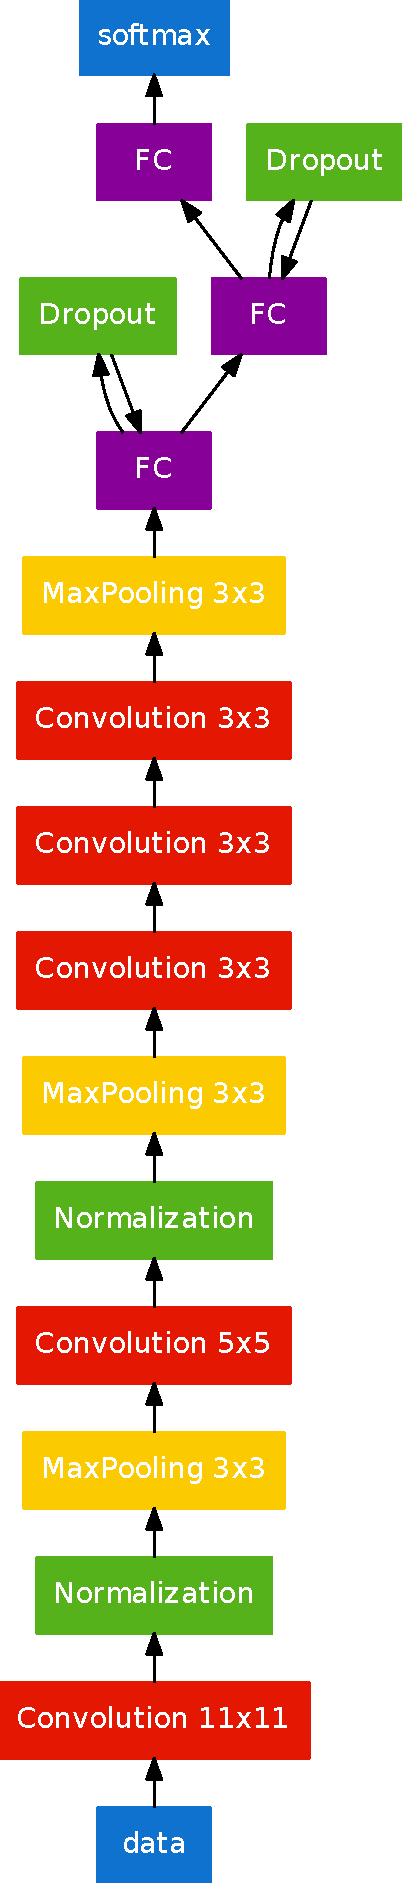
\includegraphics[height=0.65\textheight]{architectures/alexnet.pdf}
%         \subcaption{AlexNet}
%     \end{subfigure}
%     \unskip\vrule
%     \begin{subfigure}{0.21\linewidth}
%         \centering
%         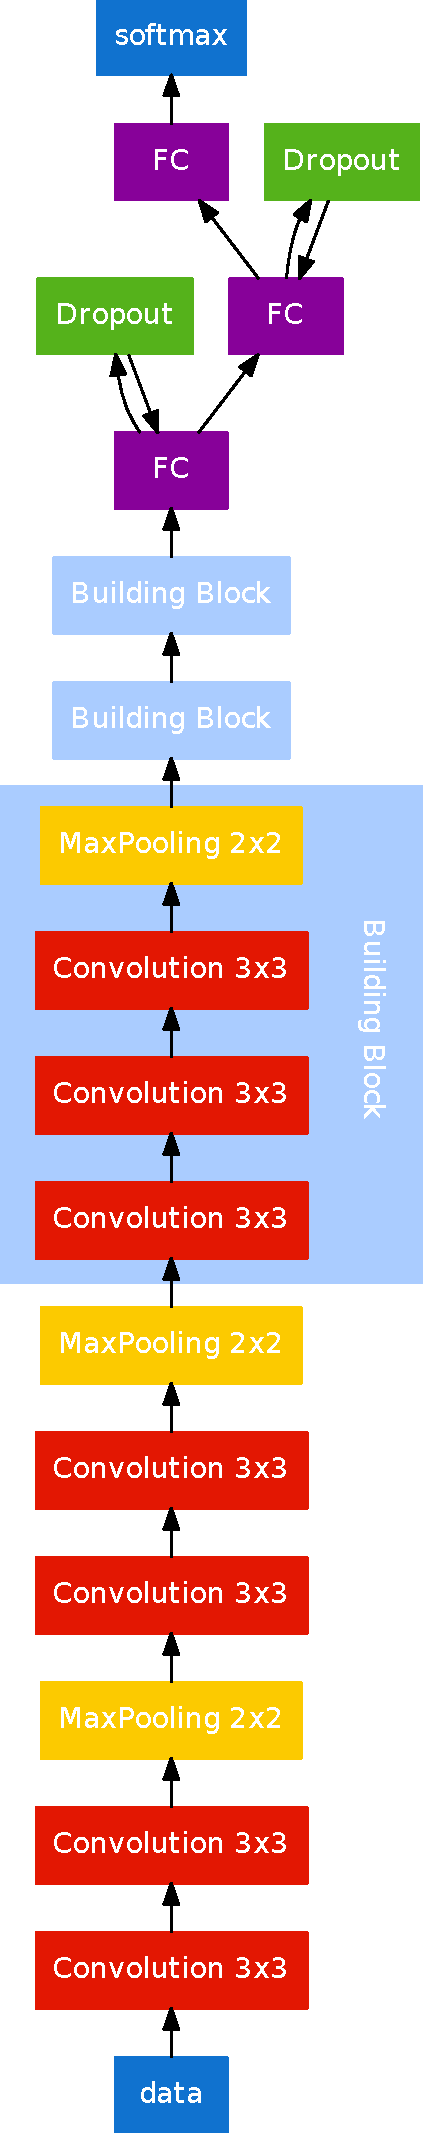
\includegraphics[height=0.65\textheight]{architectures/vgg.pdf}
%         \subcaption{VGG-16}
%     \end{subfigure}
%     \unskip\vrule
%     \begin{subfigure}{0.36\linewidth}
%         \centering
%         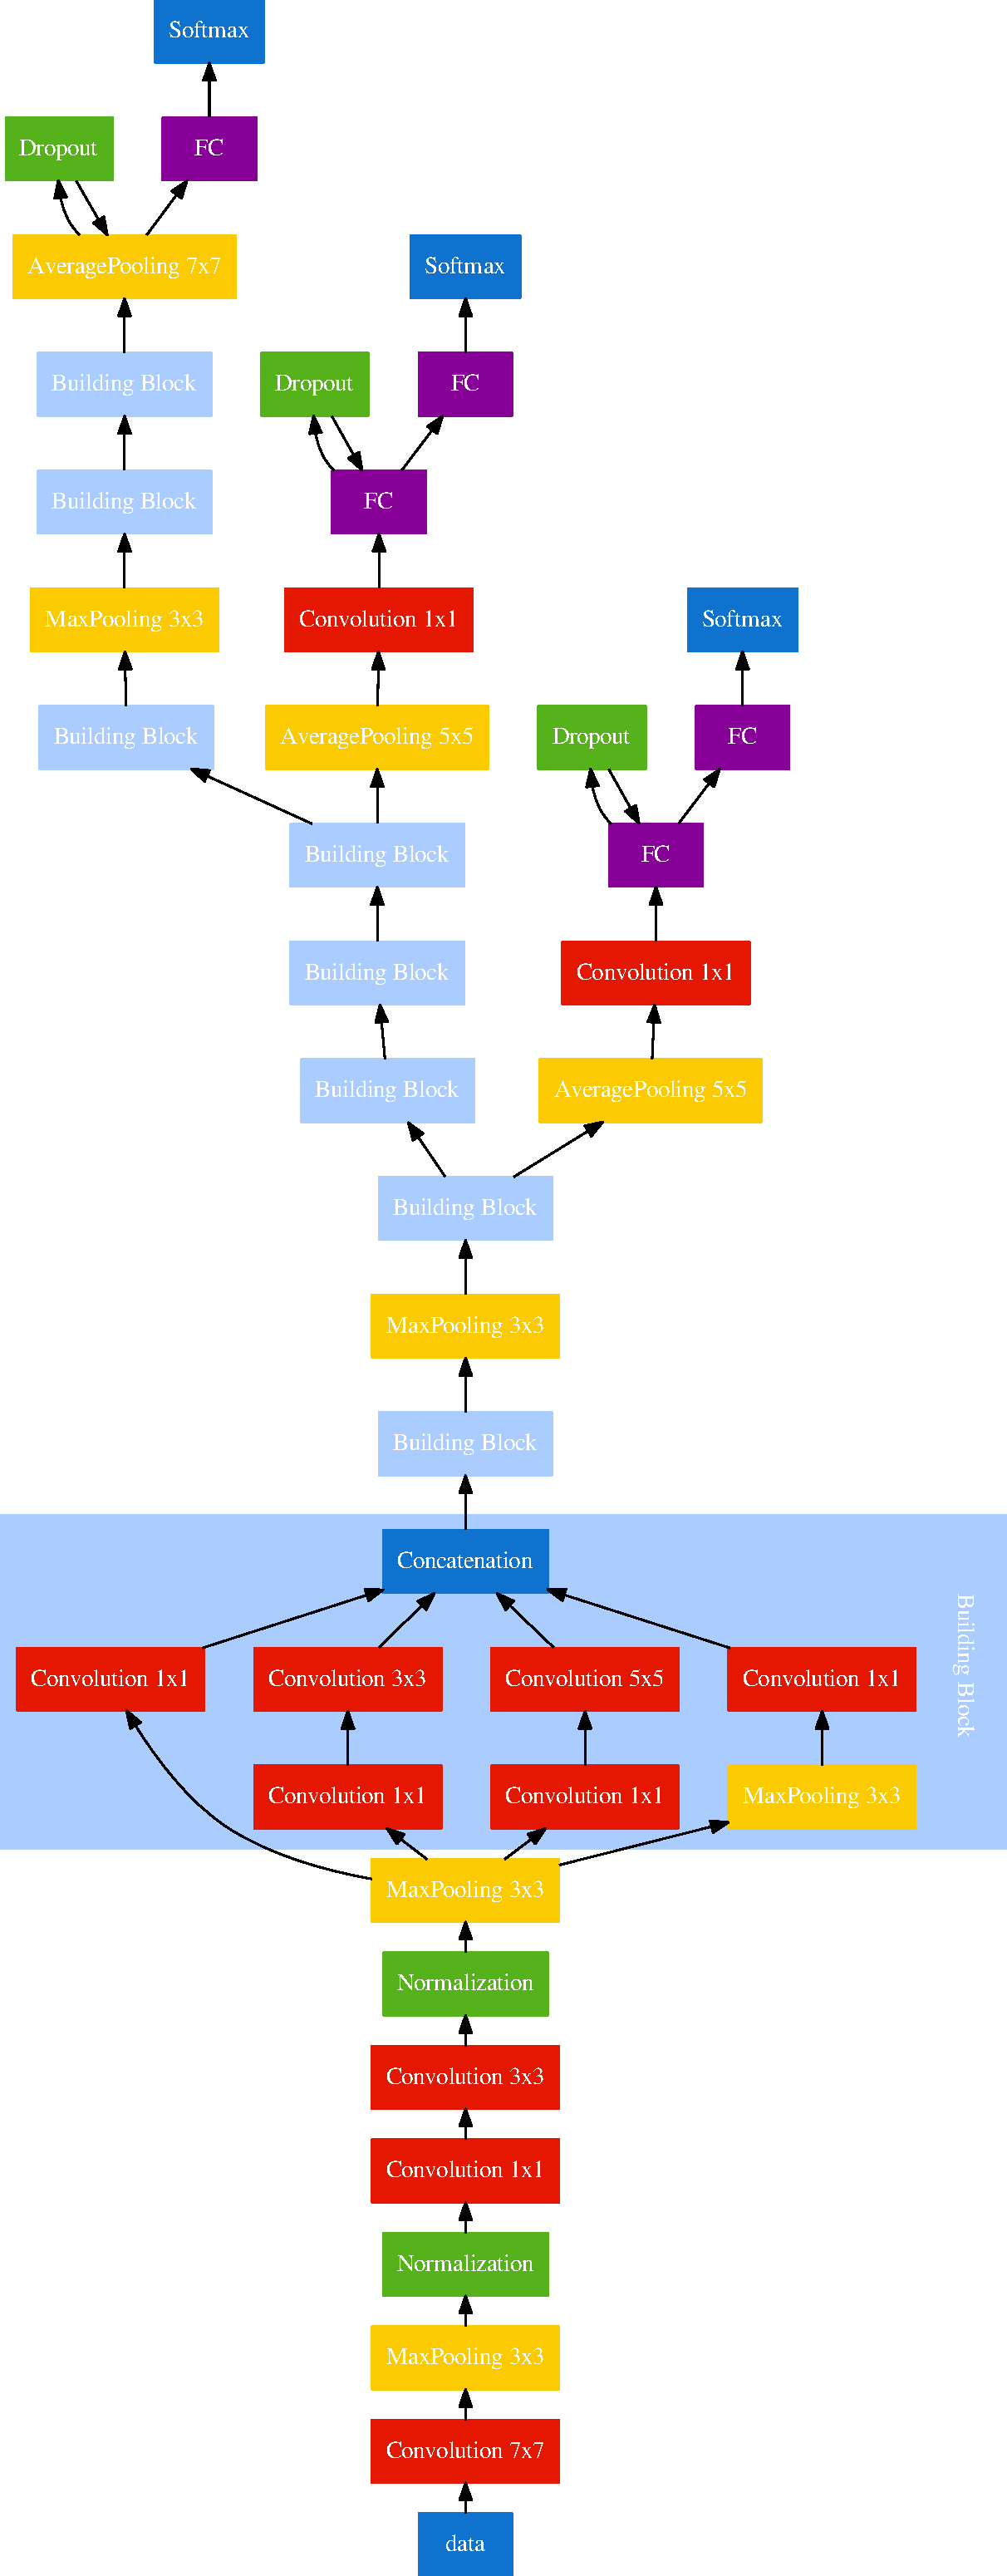
\includegraphics[height=0.65\textheight]{architectures/googlenet.pdf}
%         \subcaption{GoogLeNet}
%     \end{subfigure}
%     \unskip\vrule
%     \begin{subfigure}{0.19\linewidth}
%         \centering
%         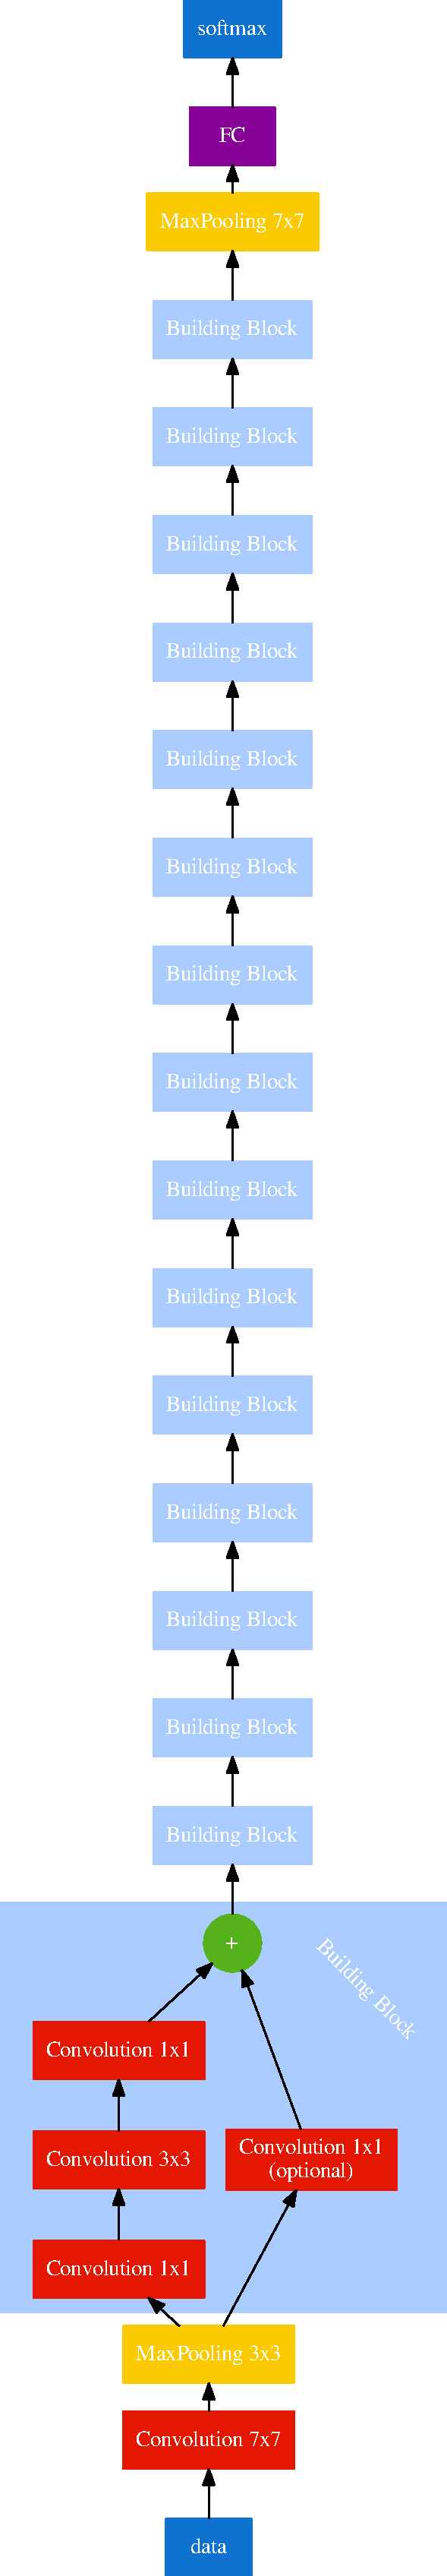
\includegraphics[height=0.65\textheight]{architectures/resnet.pdf}
%         \subcaption{ResNet-50}
%     \end{subfigure}
    
%     \caption{Deep CNN architectures used in this work}
%     \label{fig:deepcnn}
% \end{figure*}



\subsection{Network Architectures}

The deep \ac{cnn} architectures used in this paper are well known in the domain of object recognition but are not used frequently for document image classification. The networks are of very different nature (\cf~Fig.~\ref{fig:deepcnn}).

\subsubsection{\textbf{AlexNet}}
AlexNet \cite{cnn_alexnet_nips2014} is the eight-layer \ac{cnn} that won the ImageNet Large Scale Visual Recognition Challenge (ILSVRC) in 2012 \cite{russakovsky2015imagenet} by a large margin.
It employs five convolutional layers with optional pooling and local response normalization. These are then followed by three fully-connected layers and a softmax classifier (\cf~Fig.~\ref{fig:alexnet}).

\subsubsection{\textbf{VGG-16}}
VGG-16, as the name suggests is a 16-layer \ac{cnn}~\cite{simonyan2014very}. Unlike AlexNet, it uses only convolutional filters of size $3\times3$. Just like AlexNet, it has a straightforward architecture, but with $13$ convolutional layers and $3$ fully connected layers (\cf~Fig.~\ref{fig:vgg}) it is quite a bit deeper and has a repetitive pattern of layers. This architecture has won the localization category of the ILSVRC 2014.

\subsubsection{\textbf{GoogLeNet}}
GoogLeNet, just like VGG-16, won a category of the ILSVRC 2014, namely the classification category~\cite{szegedy2015going}. The architecture of this network, however, is a bit more sophisticated (\cf Fig.~\ref{fig:googlenet}). Unlike AlexNet and VGG-16, it is not just a stack of Convolution layers and Pooling layers, but rather a stack of building blocks, which themselves consist of Convolution and Pooling layers. It is therefore a Network-in-Network approach~\cite{lin2013network}. Due to its high depth, the network employs three softmax classifiers during training, to enable efficient backpropagation of the error. At test time, the two auxiliary classifiers are discarded.

\subsubsection{\textbf{Resnet-50}}
ResNets are a family of very deep \ac{cnn} architectures which make use of residual connections~\cite{he2016deep} to overcome the challenge of efficient error backpropagation. ResNet-50 is a variant of the network with $50$ layers, which, as in GoogLeNet, are grouped in building blocks (\cf~Fig.~\ref{fig:resnet}). An even deeper variant with $152$ layers won the ILSVRC classification task in 2015. Interestingly, despite its increased depth, the network has fewer parameters to fit than VGG-16.




\subsection{Preprocessing}

As the networks used in this paper require images of a fixed size as input, we first downscale all images to the expected input size of the networks. For AlexNet, the images are resized to $227\times227$ pixels, for the other networks the images are resized to $224\times224$ pixels.
Typically, when training \ac{cnn}s, the training data is augmented by resizing the images to a larger size, \eg $256\times256$ pixels and then cropping random patches of these images in the size of the network input. This approach has shown to be effective for real-world image classification~\cite{cnn_alexnet_nips2014}. In real-world images, the objects are typically close to the center of the image and therefore always contained in the random crops. However, the most discriminative parts of document images are not always close to the center of the image but reside in the outer regions, \eg the head of a letter. Therefore, we do not enlarge our training dataset in this way but train solely with images containing the entire document.

After resizing the images, we compute the mean pixel values of the training images and subtract them from all images to center the training data.

As a last preprocessing step, we convert the grayscale images to RGB images by simply copying the pixel values of the single-channel images to three channels.




\subsection{Training Details}
We train all networks using stochastic gradient descent with a momentum of $0.9$ and a learning rate that is updated every iteration to
\begin{equation}
    lr = initial\_lr * \left( 1 - \frac{iter}{max\_iter}\right) ^ {0.5}
\end{equation}
The initial learning rate is set to a value between $0.01$ and $0.0001$ depending on the network architecture, the training dataset and the weight initialization.

The number of training epochs depends on the task and ranges between $40$ and $80$ epochs.

% - training on large data set: 40 epochs, poly learn rate
% - fine tune from large to small data set: 40 epochs, poly learn rate
% - fine tune from imagenet to small data set: 80 epochs, poly learn rate
% - train from scratch to small data set: 80 epochs, poly learn rate


% The deep \ac{cnn} architecture used in the proposed approach consists of convolutional layer, maxpooling layer, \ac{relu} and the fully connected (FC) layers.
% The convolutional layers filter the input with the kernel to produce the feature maps which are either refined by the next convolutional layers or used for the classification by fully connected layers after applying the \ac{relu}.
% Pooling layers gather the overall response of the neighbouring groups of neurons in the same kernel. A window centered at the pooling location of size $n\times n$ is applied. 
% The dropout~\cite{dropout_Hinton12} layers are used to avoid any type of overfitting which may occur during the training. The dropout layer is preferred over having combinations of different models for the efficiency reasons.
% The fully connected layers are the classifiers which are used to classify the features extracted by the combination of the convolutional and the pooling layers.












% \subsection{Network Architecture}
% The architecture of the proposed neural network model (depicted in Figure~\ref{fig:deepcnn}) is inspired from~\cite{cnn_alexnet_nips2014}. 
% The model consists of eight main layers (five convolutional and the three fully connected layers). 
% The model uses the overlapping pooling \ie the windows used to summarize the outputs are overlapping.
% This can be achieved by setting the distance between the pooling units less than the size of the window.
% As depicted in Figure~\ref{fig:deepcnn} first convolutional layers processes the input of shape $227\times227\times3$.
% The first convolutional layer has $96$ kernels of size $11\times11\times3$.
% The first layer uses the stride(step size) of 4 pixels.
% The output of the first layer is then pooled to the first maxpooling layer where the average pooling and response normalization has been performed.
% The second layer has $256$ kernels of size $5\times5\times48$.
% The pooling and response normalization is perfromed for each layer except the third and the fourth layers because they are connected to each other.
% The number and the shapes of the kernels are (384, $3\times3\times256$),  (384, $3\times3\times192$) and (256, $3\times3\times192$) for third, fourth and fifth layer respectively.
% Each convolutional and fully connected layer is followed by a \ac{relu} layer.
% To avoid overfitting the dropout layer is applied to the sixth and the seventh layer which are fully connected layers.
% The eighth layer corresponds to the actual number of classes of the Tobacco-3428 Legislation dataset and hence contains $10$ output neurons corresponding to each class of the dataset.
% The output of the last layer is provided to a 10-way softmax which models a distribution over the 10 class labels. The data input and output sizes are depicted in Figure~\ref{fig:deepcnn}.


% \subsection{Learning Details}
% The objective is minimized using the stochastic gradient descent. 
% A batch size of $10$ is used.
% The learning rate, momentum and weight decay are set to $0.0001$, $0.9$ and $0.0005$ respectively.
% The weights of the network are initialized using the pretrained model\footnote{https://github.com/BVLC/caffe/tree/master/models/bvlc\_alexnet} except for the last fully connected layer.
% The training of the network has been done using Caffe\footnote{http://caffe.berkeleyvision.org/} deep learning framework~\cite{jia2014caffe}.





